\iffalse
\let\negmedspace\undefined
\let\negthickspace\undefined
\documentclass[journal,12pt,twocolumn]{IEEEtran}
\usepackage{cite}
\usepackage{amsmath,amssymb,amsfonts,amsthm}
\usepackage{algorithmic}
\usepackage{graphicx}
\usepackage{textcomp}
\usepackage{xcolor}
\usepackage{txfonts}
\usepackage{listings}
\usepackage{enumitem}
\usepackage{mathtools}
\usepackage{gensymb}
\usepackage{comment}
\usepackage[breaklinks=true]{hyperref}
\usepackage{tkz-euclide} 
\usepackage{listings}
\usepackage{gvv}                                        
\def\inputGnumericTable{}                                 
\usepackage[latin1]{inputenc}                                
\usepackage{color}                                            
\usepackage{array}                                            
\usepackage{longtable}                                       
\usepackage{calc}                                             
\usepackage{multirow}                                         
\usepackage{hhline}                                           
\usepackage{ifthen}                                           
\usepackage{lscape}
\newtheorem{theorem}{Theorem}[section]
\newtheorem{problem}{Problem}
\newtheorem{proposition}{Proposition}[section]
\newtheorem{lemma}{Lemma}[section]
\newtheorem{corollary}[theorem]{Corollary}
\newtheorem{example}{Example}[section]
\newtheorem{definition}[problem]{Definition}
\newcommand{\BEQA}{\begin{eqnarray}}
\newcommand{\EEQA}{\end{eqnarray}}
\newcommand{\define}{\stackrel{\triangle}{=}}
\theoremstyle{remark}

\newtheorem{rem}{Remark}
\begin{document}
\parindent 0px
\bibliographystyle{IEEEtran}
\title{Assignment 10.5.3\_13Q}
\author{EE23BTECH11219 - Rada Sai Sujan$^{}$% <-this % stops a space
}
\maketitle
\newpage
\bigskip
\section*{Question}
Find the sum of the first $15$ multiples of $8$. \\
\solution
\fi

\begin{table}[ht]
    \centering
    \def\arraystretch{1.5}
    \begin{tabular}{|p{2cm}|p{2.5cm}|p{2.3cm}|}
    \hline
    PARAMETER & VALUE & DESCRIPTION  \\ \hline
    $$x\brak0$$ & $$8$$ & First term \\ \hline
    $$d$$ & $$8$$ & common difference \\ \hline
    $$x(n)$$ & $$[8+8n]u\brak n$$ & General term of the series  \\ 
    \hline
  \end{tabular}

    \caption{Parameter Table1}
    \label{tab:10.5.3.1}
\end{table}
For an $AP$,
\begin{align}
    X\brak z &= \frac{ x\brak 0 }{1-z^{-1}} + \frac{dz^{-1}}{{(1-z^{-1})}^{2}}    \\
    \implies X\brak z &= \frac{8}{1-z^{-1}} + \frac{8z^{-1}}{{(1-z^{-1})}^{2}} \\
    &= \frac{8}{({1-z^{-1})}^{2}} ,\quad \abs{z}>1    \\
    y\brak{n}&=x\brak{n}\ast u\brak{n}\\
    \implies Y\brak{z}&=X\brak{z}U\brak{z}   \\
    Y\brak{z}&=\brak{\frac{8}{({1-z^{-1})}^{2}}}\brak{\frac{1}{1-z^{-1}}}  \\
    &=\frac{8}{({1-z^{-1})}^{3}} ,\quad \abs{z}>1 
\end{align}
 Using Contour Integration to find the inverse $Z$-transform,
\begin{align}
    y(14)&=\frac{1}{2\pi j}\oint_{C}Y(z) \;z^{13} \;dz  \\
    &=\frac{1}{2\pi j}\oint_{C}\frac{8z^{13}}{({1-z^{-1})}^{3}} \;dz 
\end{align}
We can observe that the pole is repeated $3$ times and thus $m=3$,
\begin{align}
    R&=\frac{1}{\brak {m-1}!}\lim\limits_{z\to a}\frac{d^{m-1}}{dz^{m-1}}\brak {{(z-a)}^{m}f\brak z}  \\
    &=\frac{1}{\brak {2}!}\lim\limits_{z\to 1}\frac{d^{2}}{dz^{2}}\brak {{(z-1)}^{3}\frac{8z^{16}}{{(z-1)}^3}}   \\
    &=4\lim\limits_{z\to 1}\frac{d^2}{dz^2}(z^{16})   \\
    &=960
\end{align}
\begin{align}
    \therefore \boxed{y(14)=960}
\end{align}
\begin{figure}[ht]
        \centering
        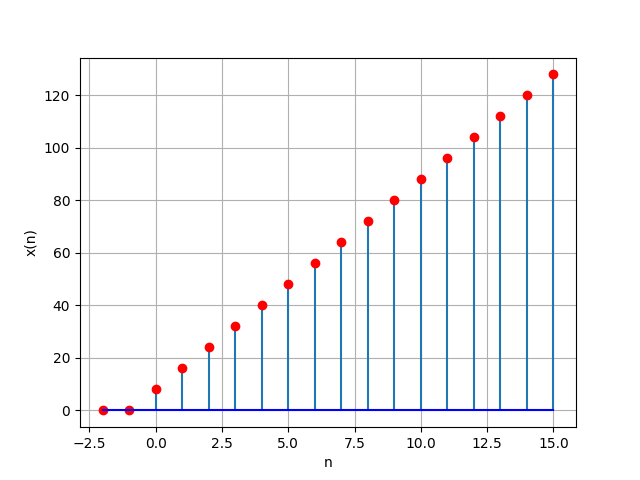
\includegraphics[width=\columnwidth]{ncert-maths/10/5/3/13/figs/a.png}
        \caption{Plot of x(n) $vs$ n}
        \label{fig:10.5.3.13.1}
    \end{figure}
    
